\documentclass{beamer}
\usetheme[titlepagelogo=minerva2,% Logo for the first page
						language=italian
                        ]{TorinoTh}
                        
\usepackage[beamer,customcolors]{hf-tikz}
\hfsetfillcolor{alerted text.fg!10}
\hfsetbordercolor{alerted text.fg}

\author{Marco Odore}
\rel{Prof. Giorgio Valentini}
\assistantsupervisor{Dr. Marco Notaro}
\title[Metodi di Ensemble Gerarchici]{Metodi di Ensemble Gerarchici per la Predizione Strutturata della Funzione delle Proteine}
\ateneo{Università Degli Studi Di Milano}
\date{10 Luglio 2018}

\begin{document}
\titlepageframe
\begin{tframe}{Il Problema della Predizione Delle Proteine}
  % 
  \begin{columns}
    %
    \begin{column}{.70\textwidth}
      \minipage[c][0.30\textheight][s]{\columnwidth}
	   \begin{itemize}	
      \item Le proteine sono polimeri (macromolecole biologiche) composte da amminoacidi, che sono codificate dai geni (porzioni di genoma) presenti nel DNA di ogni essere vivente. 

      \onslide<2->

      \item Ogni gene può codificare più proteine.

      \onslide<3->

      \item Si stima che l'essere umano possegga tra i 20.000 - 25.000 geni.
		
      \end{itemize}
      \vfill
      \onslide<4->
      \begin{tabular}{|p{0.9\textwidth}}
        Use \texttt{minipage} for top aligned images, and
        \texttt{parbox} for vertically centered images.
      \end{tabular}


      \endminipage      
    \end{column}
    %
    \begin{column}{.30\textwidth}

      % for top aligned images use minipage
      \only<1-3>{
        \minipage[c][0.8\textheight][s]{\columnwidth}

        \onslide<1->    

        \only<1-3>{
          \begin{figure}
            \centering
            \includegraphics<1>[scale=0.3]{%
              img/DNA.png} %
            \includegraphics<2-3>[scale=0.3]{%
              img/DNA.png} %
        \end{figure}}

        \only<3>{
          \begin{figure}
            \centering
            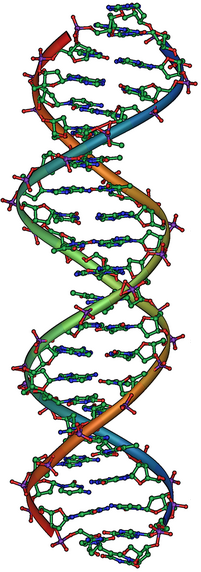
\includegraphics[scale=0.3]{%
              img/DNA.png} %
        \end{figure}}

        \endminipage
      }   

      % for vertically centered images use parbox
      \only<4>{
        \parbox[c][0.8\textheight][c]{\columnwidth}{
          \begin{figure}
            \centering
            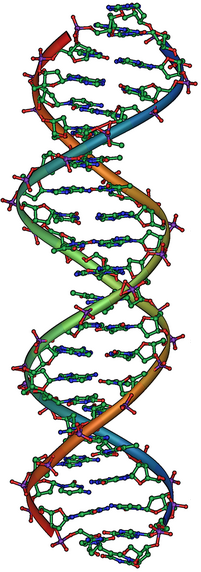
\includegraphics[scale=0.3]{%
              img/DNA.png} %
          \end{figure}
        }
      }

    \end{column}
  \end{columns}

\end{tframe}


\begin{frame}[t,fragile]{Configuration}
\begin{itemize}
\item The configuration of the standard theme is:
\begin{itemize}
\item \verb!language=italian!
\item \verb!coding=utf8x!
\item \verb!titlepagelogo=name-of-the-logo!
\item \verb!bullet=circle!
\item \verb!pageofpages=of!
\item \verb!titleline=true!
\item \verb!color=blue!
\item \verb!secondcandidate=false!
\item \verb!secondlogo=false!
\end{itemize}
\item Most of them, actually everyone except the \highlight{titlepagelogo}, can be omitted if there are no modifications
\end{itemize}
\end{frame}

\begin{frame}[fragile]{Behavior of alerts}
Each color theme requires different colors to highlight words. To insert alerts by using the \emph{itemize} environment, you can exploit:
\begin{verbatim}
\begin{itemize}
\item<+-| alert@+> Apple
\item<+-| alert@+> Peach
\end{itemize}
\end{verbatim}
For example:
\begin{itemize}
\item<+-| alert@+> Apple
\item<+-| alert@+> Peach
\end{itemize}
\end{frame}

\begin{frame}[fragile]{Another way to highlight words}
If you want to highlight your text out of the enviroment \emph{itemize}, Beamer2Thesis offers you the following possibilities:
\begin{itemize}
\item the standard command \verb!\alert{text}!: it simply highlights your \alert{text}
\item the command \verb!\highlight{text}!: it highlights your \highlight{text} setting it in italic
\item the command \verb!\highlightbf{text}!: it highlights your \highlightbf{text} setting it in bold
\end{itemize}
Of course, the color used, is set accordingly to your choice in the configuration phase.
\end{frame}

\begin{frame}[fragile]{Highlighting formulas}
\begin{itemize}
\item The package \href{http://www.ctan.org/pkg/hf-tikz}{hf-tikz} allows to highlight formulas and formula parts in Beamer with overlay specifications 
\item The adaptation of colors to the theme could be done in this way:
\begin{verbatim}
\usepackage[beamer,customcolors]{hf-tikz}
\hfsetfillcolor{alerted text.fg!10}
\hfsetbordercolor{alerted text.fg}
\end{verbatim}
\item \highlight{Two compilation runs} are required to get the right result!
\item Read the package documentation to find more options; an example will be provided in the next frame.
\end{itemize}
\end{frame}

\begin{frame}[fragile]{Highlighting formulas (II)}
\begin{itemize}
\item Example:
\[\tikzmarkin<2->{a}x+\tikzmarkin<1>{b}y\tikzmarkend{b}=10\tikzmarkend{a}\]
\item<2-> Code:
\begin{verbatim}
\[\tikzmarkin<2->{a}x+
  \tikzmarkin<1>{b}y\tikzmarkend{b}
  =10\tikzmarkend{a}\]
\end{verbatim}
\end{itemize}
\end{frame}

\begin{frame}[t,fragile]{The output}
The pdf generated, has automatically, some properties:
\begin{itemize}
\item the title
\item the name of the author
\item the subject:
\begin{itemize}
\item Thesis Presentation by using the english language
\item Presentazione Tesi di Laurea by using the italian language
\end{itemize}
\end{itemize}
This is possible thanks to the available options of hyperref. To create references in the text, use:
\begin{itemize}
\item \verb!\label{name-reference}! in the starting point
\item \verb!\ref{name-reference}! in the point you want to show the reference
\item \verb!\href{url}{name-url}! to specify web addresses
\end{itemize}
\end{frame}


\begin{frame}[fragile]{Suggestions}
\begin{itemize}
\item To realize a frame it is possible use the environment \emph{frame} with top (t), center (c) or bottom (b) alignment: I suggest you to use the top alignment; this is the basic code:
\verb!\begin{frame}[t]{title-of-the-frame}!
\begin{flushleft}
text
\end{flushleft}
\verb!\end{frame}!
\item To make things easier, it has been introduced a new environment which is able to have the top property property intrinsic:
\verb!\begin{tframe}{title-of-the-frame}!
\begin{flushleft}
text
\end{flushleft}
\verb!\end{tframe}!
\end{itemize}
\end{frame}

\begin{frame}[fragile]{Suggestions (II)}
\begin{itemize}
\item To realize the titlepage with all options, it has been introduced the command \verb!\titlepageframe!
\begin{itemize}
\item Of course, it is also possible to use the \emph{standard} approach\\
\verb!\begin{frame}[plain]!\\
\verb!\titlepage! \\
\verb!\end{frame}!
\item In this case \textbf{do not} provide a title for the frame
\end{itemize}
\item If you have to insert some code using \emph{verbatim} or \emph{listings} \textbf{do not exploit} \emph{tframe} environment, but:\\
\verb!\begin{frame}[t,fragile]{title-of-the-frame}!
\begin{verbatim}
\verb!code!
\end{verbatim}
\verb!\end{frame}!
\end{itemize}
\end{frame}

\begin{frame}[t,fragile]{Suggestions (III)}
\begin{itemize}
\item If the title does not fit in the footer box, it is possible to exploit the so called \highlight{shorttitle}; an example:
\begin{verbatim}
\title[short title]{Long title of the thesis}
\end{verbatim}
In this way the long title is just placed in the titlepage.
\item In case there are more than two supervisors or assistansupervisors, I suggest you to insert them through commands reported in \ref{secondrel} and separate names thanks to a comma.
\end{itemize}
\end{frame}

\begin{tframe}{On Facebook}
The relevance of Facebook is known to everybody: due to this reason, you can find:
\begin{itemize}
\item the group \href{https://www.facebook.com/\#!/groups/beamer2thesis/}{Beamer2Thesis}
\item the page \href{https://www.facebook.com/\#!/pages/Beamer2Thesis/112814205489099}{Beamer2Thesis}
\end{itemize} 
In this way you can post your comments, hints, suggestion and questions in more familiar way. Morevoer, you can find further examples.
\end{tframe}

\begin{tframe}{History}
Here are shortly reported the main features of the releases:
\begin{itemize}
\item basic version (2011-01-17):
\begin{itemize}
\item colors, second logo, second candidate, tframe environment, titleline, bullets, languages, separator string for slide numeration; 
\end{itemize}
\item release 2.0:
\begin{itemize}
\item third logo, assistant supervisor, new ways to highlight, new command for the titlepage, new enviroments \emph{adv} and \emph{disadv}, \XeTeX\, and \XeLaTeX\, support, blocks;
\end{itemize}
\item release 2.1:
\begin{itemize}
\item coding option, second supervisor, second assistantsupervisor;
\end{itemize}
\item release 2.2:
\begin{itemize}
\item language, short title, highlighting formulas.
\end{itemize}
\end{itemize}
\end{tframe}

\begin{tframe}{Thanks}
I would like to thank people that, with precious hints, help me:
\begin{itemize}
\item Alessio Califano
\item Alessio Sanna
\item Luca De Villa Palù
\item Mariano \emph{Dave} Graziano
\item Giovanna Turvani
\item Mattia Stefano
\item Nicola Tuveri
\item Giuliana Galati
\end{itemize}
A special thank to Claudio Beccari for very precise comments on the first version.
\end{tframe}


\end{document}
